%%% Local Variables:
%%% TeX-command-extra-options: "-shell-escape"
%%% mode: latex
%%% TeX-master: t
%%% End:
\documentclass{beamer}
\usepackage{caption}
\usepackage{minted}
\usepackage{tikz}
\usepackage{xcolor}
\usetikzlibrary{shapes.geometric, arrows}
\tikzstyle{startstop} = [rectangle, rounded corners, minimum width=3cm, minimum height=1cm,text centered, draw=black, fill=red!30]
\tikzstyle{io} = [trapezium, trapezium left angle=70, trapezium right angle=110, minimum width=1.5cm, minimum height=0.6cm, text centered, draw=black, fill=blue!30]
\tikzstyle{process} = [rectangle, minimum width=1.5cm, minimum height=0.5cm, text centered, draw=black, fill=orange!30]
\tikzstyle{decision} = [circle, radius=2.5cm, text centered, draw=black, fill=green!30]
\tikzstyle{arrow} = [thick,->,>=stealth]
\usepackage[labelformat=simple]{subcaption}

\usetheme{Singapore}
\title{Structures and All That}
\begin{document}
\begin{frame}
\titlepage
\end{frame}
\section{Compound Data}

\begin{frame}
``Here at Brymar College\\
We can get you prepared for the 31st century\\
With advanced programming and quad rendering\\
And Java plus plus plus scripting language\\
We offer advanced job placement assitance''\\
from Upgrade by Deltron 3030  
\end{frame}

\begin{frame}
  \frametitle{Data Descriptions Matter}
  We have taken a weird approach by fixating on data structured in the form of ``or'' first.
  \begin{itemize}
  \item<2-> We would say that a traffic light's state is red \textbf{\emph{or}} yellow \textbf{\emph{or}} green. I will sometimes refer to data
    in this form as defining a \emph{sum type}, but for now I will stick to saying itemization.
  \item<3-> But tons of data is written in a compound manner. A person has a head \textbf{\emph{and}} a face \textbf{\emph{and}} a body ...
    I will sometimes refer to data in this form as being a \emph{product type}, but will usually stick to saying \emph{struct}.
    When I talk about classes, I will be talking about more than compound data.
  \item<4-> Whereas with ``or'' we would check which kind of data we would have and then use a computation specific to that data, with
    products we can directly project out data.
  \item<5-> Let's say that in Java that you have some person class with a first and last name represented as strings.
  \item<6-> It is easy to define a method that returns the person's full name by concatenating the first and last name.
  \end{itemize}
\end{frame}



\begin{frame}
  \frametitle{Who Needs Structs Anyway?}
  So, why do we need compound data?
  \begin{itemize}
  \item<2-> The obvious answer is that we have programs that have some kind of compound state.
  \item<3-> Consider the simple program where we wanted to move a dot left and right.
  \item<4-> We were able to represent the state of the world as a single position number.
  \item<5-> Let's add another dimension of movement where we can now move the dot up and down.
  \item<6-> Can we represent the state of the world as a single number?
  \item<7-> If you said no, I get it! But that happens to be incorrect.
  \item<8-> We can represent a grid  with one number in the same sense that we can simulate a 10x10 2D array
    with a 100 element array.
  \end{itemize}
\end{frame}

\begin{frame}
  \frametitle{Structs Make Things Easier}
  Personally, I like doing things the easy way.
  \begin{center}
    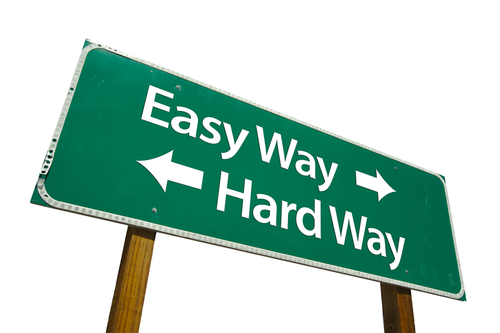
\includegraphics{images/easy-way.jpg}
  \end{center}  
\end{frame}

\defverbatim[colored]\fstName{
\begin{minted}{python}
def first_name(tup):
  return tup[0]
\end{minted}
}

\begin{frame}
  \frametitle{Unstructured Compound Data?}
  We can actually represent compound data without needing to provide names for the individual pieces of data.
  \begin{itemize}
  \item<2-> Let's consider some individual examples in Python.
  \item<3-> We can represent a Person with a first name, last name, and age with the following kind of tuple:
  \item<4-> \mintinline{python}{("Peter", "Campora", 26)}
  \item<5-> We could then define functions to act like field accesses.
  \item<6-> \fstName
  \end{itemize}
\end{frame}

\begin{frame}
  \frametitle{Data (Un)Structures}
  We can actually define other data structures in terms of things like lists.
  \begin{itemize}
  \item<2-> Let's consider defining a binary tree in terms of a python list.
  \item<3-> We can define a null node with \mintinline{python}{[]}
  \item<4-> A tree with a single root element can be \mintinline{python}{[[] 1 []]}
  \item<5-> Here's a nice balanced tree \mintinline{python}{[[[] 1 []] 2 [[] 3 []]]}
  \item<6-> This representation gets a bit ugly fast, huh?
  \item<7-> So Python gives classes (or named tuples) as a way to more easily
    define such structured data.
  \end{itemize}
\end{frame}

\begin{frame}
  \frametitle{Unstructured Data in Racket}
  Similarly, we can define data using pairs and lists in Racket.
  \begin{itemize}
  \item<2-> We can write a pair $(1, 2)$ as \mintinline{racket}{(1 . 2)}.
  \item<3-> We can write a linked list 1->2->3->4->empty as \mintinline{racket}{'(1 2 3 4)}
  \item<4-> To get the first element in the linked list, you can write:
    \mintinline{racket}{(first '(1 2 3 4))}$\hookrightarrow$ \mintinline{racket}{1}
  \item<5-> To get the rest of the linked list you can write
    \mintinline{racket}{(rest '(1 2 3 4))}$\hookrightarrow$ \mintinline{racket}{'(2 3 4)}
  \item<6-> The empty list is represented with \mintinline{racket}{'()}
    and you can check for the empty list with \mintinline{racket}{(empty? '())}
    $\hookrightarrow$ \mintinline{racket}{\#t}
  \item<7-> We will return to discussing lists in more detail later,
    since they are \emph{extremely} important.
  \item<8-> But for now, remember that we wanted to avoid the inconveniences
    given by using other existing data types to represent some piece of compound data!
  \end{itemize}
\end{frame}

\begin{frame}
  \frametitle{The Talk}
  We said that we didn't want to represent all of our compound data with
  existing structures like lists are tuples, so
  let's \emph{finally} talk about structs.
  \begin{itemize}
  \item<2-> Let's reconsider our 2 dimensional movement program.
  \item<3-> We need a natural representation for cartesian coordiantes for the state of our world.
  \item<4-> We could obviously have the state of our our world be a pair
    \mintinline{racket}{'(x . y)} or a list \mintinline{racket}{'(x  y)}
  \item<5-> But it would be better if we had piece of compound data with two fields, one field named x to represent the x coordinate and similarly a y...
  \end{itemize}
\end{frame}
\end{document}


%%% Local Variables:
%%% TeX-command-extra-options: "-shell-escape"
%%% mode: latex
%%% TeX-master: t
%%% End:
